Chaque service que nous mettons en place nécéssite implicitement d'être hébergé quelque part. N'ayant pas les moyens de nous offrir un VPS pour le déploiement de l'intégralité des services sur lesquels nous avons travaillé, nous avons pris l'opportunité de déployer ces derniers sur un serveur mis à disposition pour le projet à l'école.

Ce serveur est une machine HP de type rack 1U qui fait tourner le système d'exploitation ESXi\footnote{OS de gestion de machines virtuelles de VMware}. Grâce à cela, nous pouvons lancer des machines virtuelles sur lesquelles tourneront nos différents systèmes d'exploitation.

Bien évidemment, dans un scénario plus réaliste, nous n'aurions pas seulement un serveur, mais plusieurs. Les ressources de l'école nous limite à n'utiliser qu'un serveur physique. Nous considèrerons alors que chaque système d'exploitation tournant sur ESXi soit en fait un serveur physique qui va, plus tard, faire partie d'un "cluster". Je vais revenir sur ce terme là un peu plus tard.

\section{Virtualisation des services}

\begin{figure}[H]
    \centering
    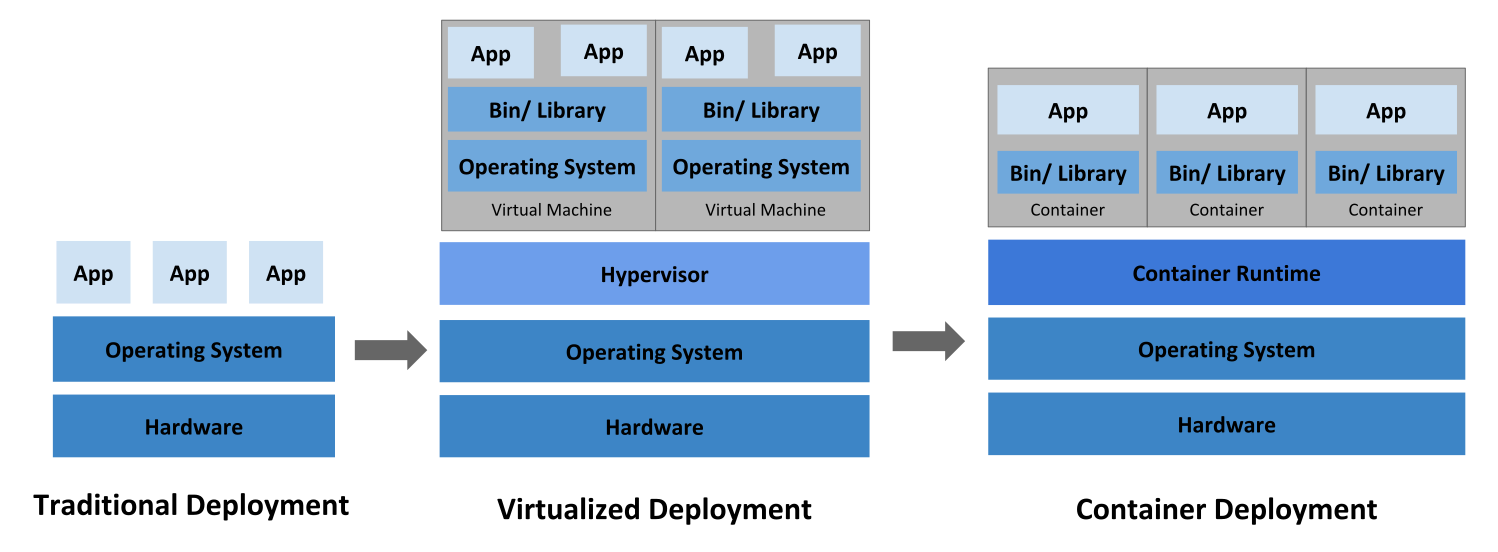
\includegraphics[width=\textwidth]{./img/container_evolution.png}
    \caption{Évolution du déploiement d'applications \cite{shavidissa2019}}
    \label{fig:container_evolution}
\end{figure}

Traditionnellement, lorsqu'une application devait être déployée et rendue utile au grand public, elle était simplement exécutée sur le système d'exploitation de la machine physique hôte. Ce "déploiement traditionnel", qui, à la surface, semblait simple, posait en fait, au long terme, bien des problèmes. On peut citer des problèmes de sécurité car l'application cohabiterai avec d'autres applications ou bien des problèmes de scalabilité, où les applications sont limités au niveau des ressources qu'offre le hardware de la machine, mais aussi des problèmes où l'application dépendrait de l'intégrité du système dans lequel elle est installée.

Pour palier à tout ça, une des solutions est de travailler avec des machines virtuelles. Un hyperviseur va pouvoir orchestrer différents systèmes d'exploitation dans lesquels résideront les services que nous souhaitons déployer. Ainsi, chaque service sera isolé des autres. De plus, il est possible de mettre en place un système qui, en cas de défaut d'une instance d'un service ou en cas de demande saturée du service, il est possible de lancer, à la volée, une machine virtuelle qui ferait tourner ce service. Rendant ainsi possible un load balancing des requêtes envers ce service. Un des seuls soucis avec tout ça, c'est que l'utilisation des machines virtuelles présente un overhead plutôt conséquent.

La solution que nous avons opté découle des deux solutions ci-dessus. Elle améliore le service en le redant:

\begin{itemize}
    \item plus isolé
    \item plus facilement instanciable
    \item moins coûteux en terme d'overhead
\end{itemize}

Le principe est d'avoir plusieures machines présentant chacune leur propre système d'exploitation (ici, Linux\footnote{ou plus précisément, Ubuntu 23.04}). Dans ces systèmes d'exploitation tourneront des moteurs de containerization, comme Docker.

\subsection{Docker}

Comme dit précédemment, La technologie de containerization que nous allons utiliser s'appelle Docker. Elle permet de "construire" notre propre container avec le service que nous souhaitons déployer. Il restera alors à dire à Docker de déployer un service untel et le service se déploiera\dots N'est-ce pas ?

Certains d'entre vous me diront "Mais Flo, qu'en est-il de l'orchestration des différents services, tu sais, l'avantage que nous présentais le deuxième point ?". Malheureusement, jeune padawan, Docker ne nous permets pas ça. Il permet d'isoler un environnemnt mais sur qu'une seule machine. Travailler en harmonie avec d'autres moteurs docker reste impossible\dots ou du moins sans notre dernière solution.
\section{Kubernetes}


